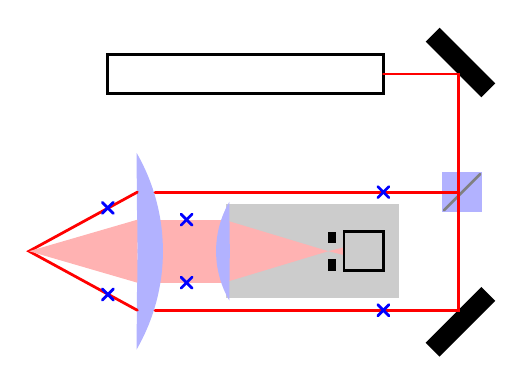
\begin{tikzpicture}
    \begin{scope}[x={(0mm,300mm)},y={(0mm,185mm)},line width=1pt,cap=round,rotate=-90]
        % bounding box
        %\draw[black] (190mm,70mm) rectangle (245mm,140mm);

        % laser and cable
        \draw[black] (200mm,120mm) rectangle (205mm,85mm);

        % mirror 1
        \fill[black,rotate around={45:(197.5mm,126.25mm)}] (197.5mm,125mm) rectangle (207.5mm,127.5mm);

        % beam splitter
        \fill[blue!30]  (215mm,127.5mm) rectangle (220mm,132.5mm);
        \draw[black!50] (215.2mm,132.3mm) -- (219.8mm,127.7mm);
        %\node at (215mm,120mm) {\footnotesize{1}};

        % mirror 2
        \fill[black,rotate around={-45:(237.5mm,126.25mm)}] (227.5mm,125mm) rectangle (237.5mm,127.5mm);

        % housing around detector and L2
        \fill[black!20] (219mm,122mm) rectangle (231mm,100mm);


        % dispersed light below lenses
        \fill[red!30] (221mm,90mm) rectangle (229mm,99.75mm);
        \fill[red!30] (221mm,99.75mm) -- (225mm,113mm) -- (229mm,99.75mm);
        \fill[red!30] (225mm,113mm) -- (224.5mm,115mm) -- (225.5mm,115mm);

        % detector and power cable and signal cables
        \draw[black] (222.5mm,120mm) rectangle (227.5mm,115mm);

        % aperture
        \fill[black] (222.5mm,114mm) rectangle (224mm,113mm);
        \fill[black] (226mm,114mm) rectangle (227.5mm,113mm);

        % lens L2
        \fill[blue!30] (225.25mm,100.5mm) -- (225mm,98.75mm) arc[start angle=-90,delta angle=-30,radius=12.5mm]  -- cycle;
        \fill[blue!30] (224.75mm,100.5mm) -- (225mm,98.75mm) arc[start angle=-90,delta angle=30,radius=12.5mm] -- cycle;

        % lens L1
        \fill[blue!30] (224.75mm,88.75mm) -- (225mm,92mm) arc[start angle=90,delta angle=-30,radius=25mm] -- cycle;
        \fill[blue!30] (225.25mm,88.75mm) -- (225mm,92mm) arc[start angle=90,delta angle=30,radius=25mm]  -- cycle;

        % Laser beams
        % laser -> L1
        \draw[red] (202.5mm,120mm) -- (202.5mm,129.5mm) -- (217.5mm,129.5mm) -- (217.5mm,91mm);
        % L1 -> L1
        \draw[red] (217.5mm,88.75mm) -- (225mm,75mm) -- (232.5mm,88.75mm);
        % L1 -> beam splitter
        \draw[red] (232.5mm,91mm) -- (232.5mm,129.5mm) -- (217.5mm,129.5mm);
        % particle -> L1 (dispersion)
        \fill[red!30] (225mm,75mm) -- (229mm,88.75mm) -- (221mm,88.75mm);

        % forward beam, left
        \draw[blue,rotate around={45:(217.5mm,120mm)}] (216.5mm,120mm) -- (218.5mm,120mm);
        \draw[blue,rotate around={-45:(217.5mm,120mm)}] (216.5mm,120mm) -- (218.5mm,120mm);

        % forward beam, right
        \draw[blue,rotate around={45:(232.5mm,120mm)}] (231.5mm,120mm) -- (233.5mm,120mm);
        \draw[blue,rotate around={-45:(232.5mm,120mm)}] (231.5mm,120mm) -- (233.5mm,120mm);

        % forward beam, after L1, left
        \draw[blue,rotate around={45:(219.5mm,85mm)}] (218.5mm,85mm) -- (220.5mm,85mm);
        \draw[blue,rotate around={-45:(219.5mm,85mm)}] (218.5mm,85mm) -- (220.5mm,85mm);

        % forward beam, after L1, right
        \draw[blue,rotate around={45:(230.5mm,85mm)}] (229.5mm,85mm) -- (231.5mm,85mm);
        \draw[blue,rotate around={-45:(230.5mm,85mm)}] (229.5mm,85mm) -- (231.5mm,85mm);

        % backwards beam, left
        \draw[blue,rotate around={45:(221mm,95mm)}] (220mm,95mm) -- (222mm,95mm);
        \draw[blue,rotate around={-45:(221mm,95mm)}] (220mm,95mm) -- (222mm,95mm);

        % backwards beam, right
        \draw[blue,rotate around={45:(229mm,95mm)}] (228mm,95mm) -- (230mm,95mm);
        \draw[blue,rotate around={-45:(229mm,95mm)}] (228mm,95mm) -- (230mm,95mm);
    \end{scope}
\end{tikzpicture}
